\section{Previous Work}
Last year, Pedro Ferreira developed a study, present in \cite{pedro-report}, addressing the evolution of the electric vehicles adoption in Portugal, from a perspective of competitiveness between companies through a series of factors such as: \textbf{Average Quality}, \textbf{Range}, \textbf{Top Speed}, among others.

This study focused on the perspective of market share between different manufactures in function of their weaknesses and strengths. The dynamic model that was implemented in this work can be seen in figure \ref{fig:vensim-model-pedro}.

\begin{figure}[htbp]
\centerline{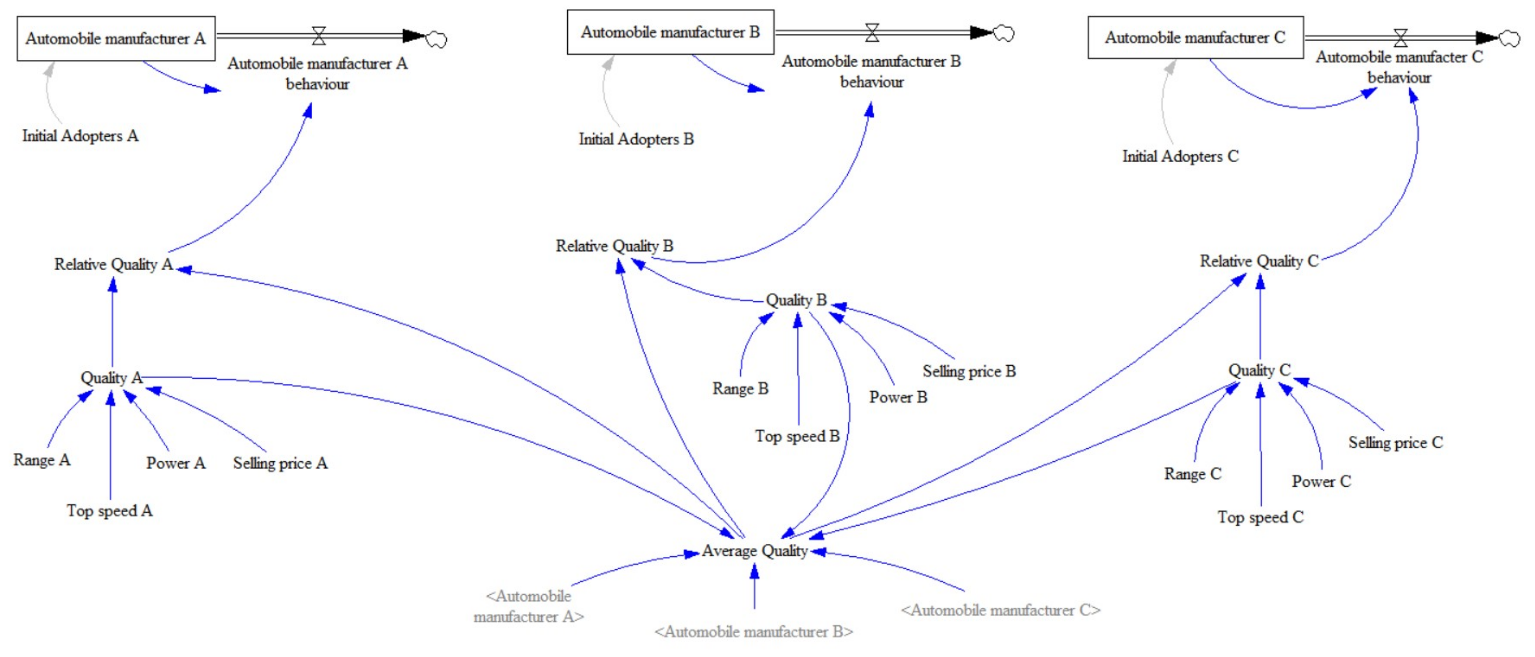
\includegraphics[width=0.9\linewidth]{img/vensim-model-pedro.png}}
\caption{Stock and Flow Diagram of Electric Vehicles adoption. Source: \cite{pedro-report}}
\label{fig:vensim-model-pedro}
\end{figure}

In this study, the author analyzed the market share evolution, average quality and relative quality of electric vehicles throughout a period of 12 months. This analysis allowed the author to conclude that, given the studied scenario, the most important decision factors would be: \textbf{price} and \textbf{charging time} and that the manufacturer with the best balance between these two factors, regardless the initial adopters, would eventually take up most of the market share of electric vehicles.

Although this study brings helpful insight to what factors could make a specific manufacturer succeed over the others, it fails to provide an understanding on how the EV market would evolve over the next years taking into consideration important factors to the consumers' choice. As I said in section \ref{section:intro}, environmental concerns are more and more present in today's society and it's helpful to better understand how the EV market will evolve to better grasp what will be the contribution of transport vehicles to the overall reduction of CO2 emissions and what are the factors that most dictate the growth of this market. 

Having that said, this work builds on the insights provided in \cite{pedro-report} and enhances it with a more global vision of the growth of the entire EV market that allows to grasp a broad perspective and have a means of comparing with the market of internal combustion vehicles.

\clearpage
